\documentclass[12pt,a4paper]{article}
\usepackage{cmap}
\usepackage[utf8]{inputenc}
\usepackage[T1,T2A]{fontenc}
\usepackage[english,russian]{babel}
\usepackage{amsmath,booktabs,array,graphicx}
\usepackage{caption,float,qrcode}
\usepackage{geometry,hyperref,indentfirst}
\geometry{margin=25mm}
\hypersetup{unicode=true,colorlinks=true,urlcolor=blue,linkcolor=black}
\setlength{\parindent}{1.25cm}
\setlength{\parskip}{0pt}
\setlength{\emergencystretch}{2em}
\DeclareCaptionLabelSeparator{emdash}{\space---\space}
\captionsetup[figure]{justification=centering,singlelinecheck=false,labelsep=emdash}
\addto\captionsrussian{\renewcommand{\figurename}{Рис.}}
\linespread{0.96}
\makeatletter
\newcommand{\inputrows}[1]{\@@input #1 }
\makeatother
\begin{document}
\hypersetup{pageanchor=false}
\begin{titlepage}
\begin{center}
{\large МОСКОВСКИЙ АВИАЦИОННЫЙ ИНСТИТУТ\\
(НАЦИОНАЛЬНЫЙ ИССЛЕДОВАТЕЛЬСКИЙ УНИВЕРСИТЕТ)}
\vspace{18pt}
{\large Факультет информационных технологий и прикладной математики}

{\large Кафедра вычислительной математики и~программирования}
\vfill
{\large\textbf{Лабораторная работа №13 по курсу\\ «Информационный поиск»}}
\vspace{12mm}

{\large\textbf{Текстовое ранжирование TF-IDF}}
\vfill
\begin{flushright}
\begin{tabular}{@{}r@{:\hspace{0.6em}}l@{}}
\textit{Студент} & К.\,А. Арусланов\\
\textit{Группа} & М8О-403Б-23\\
\textit{Преподаватель} & А.\,А. Кухтичев\\
\textit{Дата} & 08.11.2026\\
\textit{Оценка} &
\end{tabular}
\end{flushright}
\vfill
Москва, 2026
\end{center}
\end{titlepage}
\hypersetup{pageanchor=true}
\setcounter{page}{2}
\tableofcontents
\newpage

\section{Постановка задачи}
Добавить в поисковую систему ранжирование документов на основе TF-IDF.
Вместо порядка по идентификатору выдавать сначала документы с большей
оценкой соответствия запросу. Реализовать запросы из обычных слов,
ограничение выдачи top-$k$, интерфейс командной строки и веб-форму.
Проверить численную правильность оценок, измерить время и дополнительный
объём индекса, рассмотреть изменение первых результатов.

Основные структуры и алгоритмы поиска реализуются на C++ без STL-контейнеров.
Python используется для веб-обвязки, запуска экспериментов и подготовки
таблиц. Входные и выходные данные имеют кодировку UTF-8.

\section{Метод решения}
\subsection{От булева поиска к весам терминов}
Булев поиск определяет, подходит документ запросу или нет. Если результатов
много, порядок по ID не помогает выбрать наиболее подходящие публикации.
Для ранжирования документ и запрос представлены разреженными векторами
терминов. Выбрана схема \texttt{lnc.ltc} из лекции о текстовом ранжировании
(\texttt{lesson-09}, слайды 41--43).

Частота $tf_{t,d}$ равна числу вхождений термина $t$ в документ $d$.
Координаты из ЛР10 позволяют посчитать её без повторного чтения корпуса:
вхождения в заголовке и основном тексте складываются. В этой работе поля
имеют одинаковый вес. Логарифмическая частота задаётся как
\[
 L(x)=\begin{cases}1+\log_{10}x,&x>0,\\0,&x=0.\end{cases}
\]
Так повторение слова увеличивает вес, но увеличение частоты в десять раз
не означает десятикратного увеличения вклада в оценку.

Документная частота $df_t$ --- число документов, содержащих термин,
а $N$ --- число всех документов снимка, включая пустые. Обратная
документная частота равна $idf_t=\log_{10}(N/df_t)$.
Она отличается от общего числа вхождений слова в корпус.
Редкий термин имеет больший IDF; термин с $df_t=N$ имеет нулевой IDF.

\subsection{Схема lnc.ltc и косинусная нормировка}
В обозначении \texttt{lnc.ltc} три символа до точки относятся к документу,
три после неё --- к запросу. \texttt{l} означает логарифмический TF,
\texttt{n} --- отсутствие множителя IDF, \texttt{t} --- IDF,
\texttt{c} --- косинусную нормировку. Таким образом,
\[
 w_{t,d}=L(tf_{t,d}),\qquad w_{t,q}=L(tf_{t,q})\,idf_t,
\]
\[
 \|d\|=\sqrt{\sum_{t\in V}w_{t,d}^2},\qquad
 \|q\|=\sqrt{\sum_{t\in q}w_{t,q}^2},\qquad
 score(d,q)=\frac{\sum_{t\in q\cap d}w_{t,d}w_{t,q}}{\|d\|\,\|q\|}.
\]
Норма документа считается по \emph{всему} словарю пространства $V$.
Если ограничить её словами запроса, дополнительные слова документа
перестанут влиять на нормировку, и получится другая модель.
Оценка является косинусным сходством преобразованных векторов,
а не вероятностью релевантности.

В тексте слайда 42 нормировка описана неточно; в реализации используется
значение \texttt{c} из таблицы на слайде 41 и нормированный пример слайда 43.
Словам запроса, отсутствующим в словаре корпуса, не соответствует ось:
они исключаются из расчёта. Если после этого норма запроса равна нулю,
выдача пуста. Документы с нулевой оценкой не включаются в результат.

\subsection{Построение и использование норм}
Для каждого термина исходного координатного индекса последовательно
читаются его вхождения и группируются по документам. По полученному TF
к сумме квадратов соответствующего документа добавляется $L(tf)^2$.
Одновременно проверяется совпадение DF с булевым индексом.
После полного прохода из сумм извлекаются квадратные корни.

Один физический индекс содержит пространства словоформ и лемм.
Нормы для них считаются отдельно. При неоднозначной лемматизации каждая
различная альтернатива является отдельным термином, как в предыдущих работах.
Если альтернативы нескольких слов запроса совпали, они объединяются
в одну ось с суммированием query TF.

Расширение хранит два массива норм double и заголовок 80 байт.
В нём записаны версия формулы, размеры, FNV-64 и привязка к исходным
заголовкам индекса. Расширение совместимо с исходной и соответствующей
упакованной копией. При открытии проверяются привязка, размеры,
контрольная сумма и допустимость всех значений.
Незавершённая сборка помечается \texttt{INCOMPLETE} и не открывается.

\subsection{Поиск и отбор top-k}
Запрос токенизируется; при необходимости выполняется лемматизация.
После объединения одинаковых терминов вычисляются веса и норма запроса.
Координаты каждого его термина читаются последовательно. Для очередного
документа подсчитывается TF и увеличивается накопленная оценка.
Затем оценки делятся на заранее рассчитанные нормы документов.

Накопитель содержит $N$ значений double. Для top-$k$ используется собственная
ограниченная двоичная куча: в корне находится худший из отобранных результатов.
Лучший кандидат заменяет его с восстановлением кучи. В конце куча сортируется
по убыванию оценки; при точном равенстве раньше идёт меньший исходный ID.
Поддерживаются произвольные 64-битные ID, включая максимальное значение.

Память основных массивов составляет $16N$ байт норм и $8N$ байт оценок,
то есть 11,49 МБ на данном корпусе. Дополнительно нужны буферы, словарь
лемматизатора и $O(k)$ памяти результатов. Время состоит из чтения координат
терминов запроса, обхода массива $O(N)$ и отбора $O(M\log k)$,
где $M$ --- число документов с положительной оценкой.
Полный словарь и координатный индекс в память не загружаются.

В CLI выбран режим \texttt{--ranking tfidf}; запросы читаются по строкам
stdin, ответы выдаются в JSONL. Поле \texttt{score} содержит оценку,
\texttt{total} --- полное число положительных совпадений,
\texttt{--limit} ограничивает только число показанных результатов.
Веб-форма вызывает тот же C++-поиск и позволяет выбрать способ выдачи.
В режиме TF-IDF слова образуют «мешок слов»: порядок и кавычки
не задают обязательную фразу. Булев и цитатный поиск доступны отдельно.

\section{План и результаты тестирования}
Для численной проверки используется небольшой корпус с заранее известными
частотами. Независимый эталон в GoogleTest строит полные векторы из текстов,
вычисляет DF, TF-IDF и косинус, а затем полностью сортирует результаты.
Основной алгоритм сравнивается с ним с допуском $10^{-12}$.

План включает следующие группы проверок:
\begin{enumerate}
\item Однословные и многословные запросы, повторение слов, неизвестные слова,
      одинаковые частоты и объединение вхождений заголовка и текста.
\item Норма по всему словарю, включая слова вне запроса; влияние лишних слов
      на итоговую оценку документа.
\item Точное совпадение top-$k$ с префиксом полной сортировки,
      $k=0$, равные оценки и большие ID. Отдельный корпус из 1200 документов
      проверяет кучу для $k=1,7,20,1000$.
\item Пустой корпус, пустые документы, отсутствие совпадений и запрос только
      из терминов с нулевым IDF: отсутствие деления на ноль и NaN.
\item Отдельные нормы лемм, неоднозначные разборы и объединение альтернатив
      в запросе; идентичность оценок исходного и сжатого индексов.
\item Повреждённые, усечённые, чужие и незавершённые нормы; недопустимый UTF-8,
      ограничения длины, последовательность запросов с восстановлением после ошибки.
\item Передача параметров из веб-формы, UTF-8, вывод оценок и выбор TF-IDF
      через настоящий HTTP-запрос к тестовому серверу.
\end{enumerate}

Группа ЛР13 содержит 11 GoogleTest, проверку CLI help и 3 Python-теста.
Полная регрессия завершилась успешно: 144 CTest и 286 Python-тестов;
6 интеграционных проверок MongoDB пропущены.
Журнал прогона приложен в \path{lab13/tests.txt}.

\section{Результаты}
\subsection{Корпус и условия измерений}
Использован тот же снимок из 478\,833 игровых публикаций, что в предыдущих
работах. В двух пространствах суммарно 2\,545\,616 терминов и
335\,548\,564 координаты. Построение норм заняло 51,140 с, включая полную
проверку исходных булева и координатного индексов. Это один запуск,
а не медиана. Размер расширения --- 7\,661\,408 байт, около 7,66 МБ.

Поиск выполнялся по упакованному VB-индексу. Для измерения времени в каждом
пространстве сравнивались OR с порядком по ID и TF-IDF по тем же словам
запроса. OR выбран здесь потому, что для заданных запросов он перебирает
тот же набор документов, которым TF-IDF назначает положительную оценку.
Для сравнения первых результатов дополнительно выполнен более строгий
булев запрос с AND; его число найденных документов показано отдельно.
Проведено семь раундов, порядок режимов и запросов чередовался.
Каждый процесс выполнял прогревочный пакет и затем измеряемый пакет.
Кэш ОС не очищался. Приведены медианы времени внутри C++:
нормализация запроса, чтение списков, расчёт оценок и отбор результатов.
Открытие индекса, загрузка морфологии и норм, чтение метаданных выдачи
и вывод JSON в это время не входят.

\subsection{Время поиска}
В таблице приведены результаты для словоформ. Для выбранных запросов
число кандидатов OR совпало с числом положительных оценок TF-IDF;
оно не зависит от ограничения top-10.
\begin{center}
\small
\begin{tabular}{@{}lrrr@{}}
\toprule
Запрос & Кандидатов & OR/ID, мс & TF-IDF, мс\\
\midrule
\inputrows{lab13/query_rows.tex}
\bottomrule
\end{tabular}
\end{center}

Ранжирование требует больше работы, чем перечисление булева объединения:
нужно восстановить TF из координат и вычислить оценки. Особенно заметна
разница на \texttt{god of war}, где частое слово \texttt{of} порождает длинный
список. Поэтому TF-IDF здесь улучшает порядок выдачи ценой времени поиска.

Для лемм запросы «игры» и «игрой» дали одинаковое число кандидатов
230\,075; медианы составили 67,103 и 63,765 мс соответственно.
По словоформам это разные запросы: 149\,495 и 22\,588 кандидатов.
Все оценки и top-10 сохранялись между повторениями; исходный и сжатый
форматы дополнительно сопоставлены в численных автотестах.

\subsection{Примеры выдачи и оценка по заголовкам}
Для запроса \texttt{doom eternal} в TF-IDF первыми стали:
\begin{center}
\small
\begin{tabular}{@{}p{115mm}r@{}}
\toprule
Заголовок & Оценка\\
\midrule
Doom Eternal --- Мнение & 0,81278\\
Сравнение графики Doom vs Doom Eternal & 0,67033\\
5 подтвержденных оружий в Doom Eternal & 0,57472\\
Doom Eternal --- 20 минут захватывающего геймплея & 0,54836\\
Fallout 76 --- Новая система перков и отличный DOOM Eternal & 0,44219\\
\bottomrule
\end{tabular}
\end{center}
Более строгий запрос \texttt{doom AND eternal} нашёл 1\,392 документа
против 9\,170 документов с положительной оценкой TF-IDF.
Среди первых пяти результатов AND по ID два заголовка прямо называли
Doom Eternal, в первых пяти TF-IDF --- все пять. Таким образом, оба
режима способны найти публикации по игре, но формируют разные первые
результаты. Общее число результатов здесь нельзя считать показателем
релевантности: AND требует оба слова, а TF-IDF допускает одно совпадение.

Для небольшой иллюстративной оценки взяты три запроса по названиям игр.
Помощником вручную размечено объединение первых пяти результатов AND/ID и TF-IDF
по видимым заголовкам. Метка 1 означает, что заголовок прямо называет искомую
игру, включая русское написание; метка 0 --- что тема из заголовка не установлена.
Для каждого режима рассчитана доля меток 1 в первых пяти результатах (P@5).
\begin{center}
\begin{tabular}{@{}lrr@{}}
\toprule
Запрос & AND/ID & TF-IDF\\
\midrule
doom eternal & 0,40 & 1,00\\
god of war & 0,80 & 1,00\\
cyberpunk 2077 & 0,60 & 1,00\\
\midrule
Среднее & 0,60 & 1,00\\
\bottomrule
\end{tabular}
\end{center}
Это оценка соответствия заголовков теме на трёх примерах. Полные тексты
не размечались, запросы не составляют представительную независимую выборку.
По этим результатам нельзя заключить, что общая точность поиска равна 1.
Разметка сохранена вместе с ID и заголовками, поэтому расчёт можно повторить.

На рис.~\ref{fig:codes_bool} и \ref{fig:codes_tfidf} показан ещё один
реальный запрос в пространстве лемм. Булев режим выполняет
\texttt{чит AND коды AND gta} и находит 6 документов. Режим TF-IDF
обрабатывает \texttt{чит коды gta} как запрос из слов и находит 18\,743
документа с положительной оценкой. В булевой первой пятёрке по ID есть
«Gears of War», «Наши истории» и статья о чит-кодах вообще; у TF-IDF
первыми идут публикации, в заголовках которых упоминаются GTA и читы
или коды. Один документ, ID~431\,639, присутствует в обеих выдачах;
TF-IDF ставит его на первое место. Скриншоты показывают порядок и число
результатов в отдельных запусках веб-интерфейса; время на них не является
медианой измерений из предыдущей таблицы.

\begin{figure}[H]
\centering
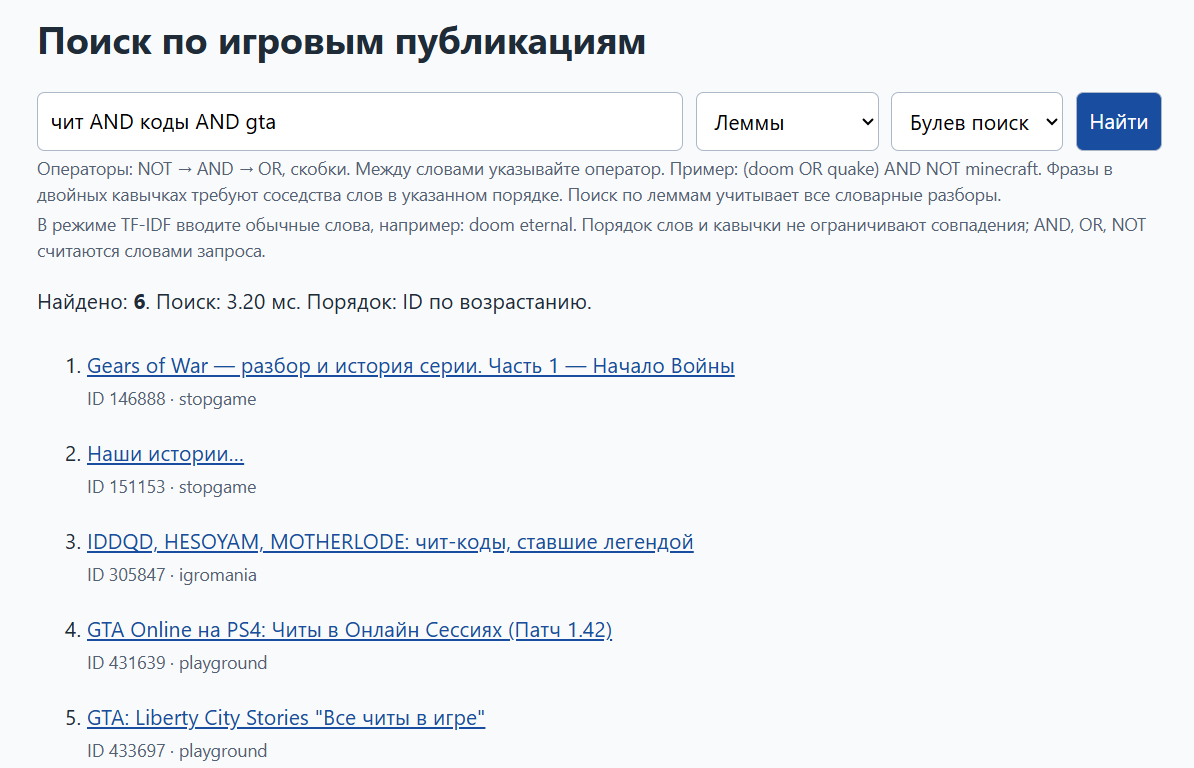
\includegraphics[width=0.96\linewidth]{img/codes_bool.png}
\caption{Булев запрос по леммам: все три слова обязательны, выдача по ID}
\label{fig:codes_bool}
\end{figure}

\begin{figure}[H]
\centering
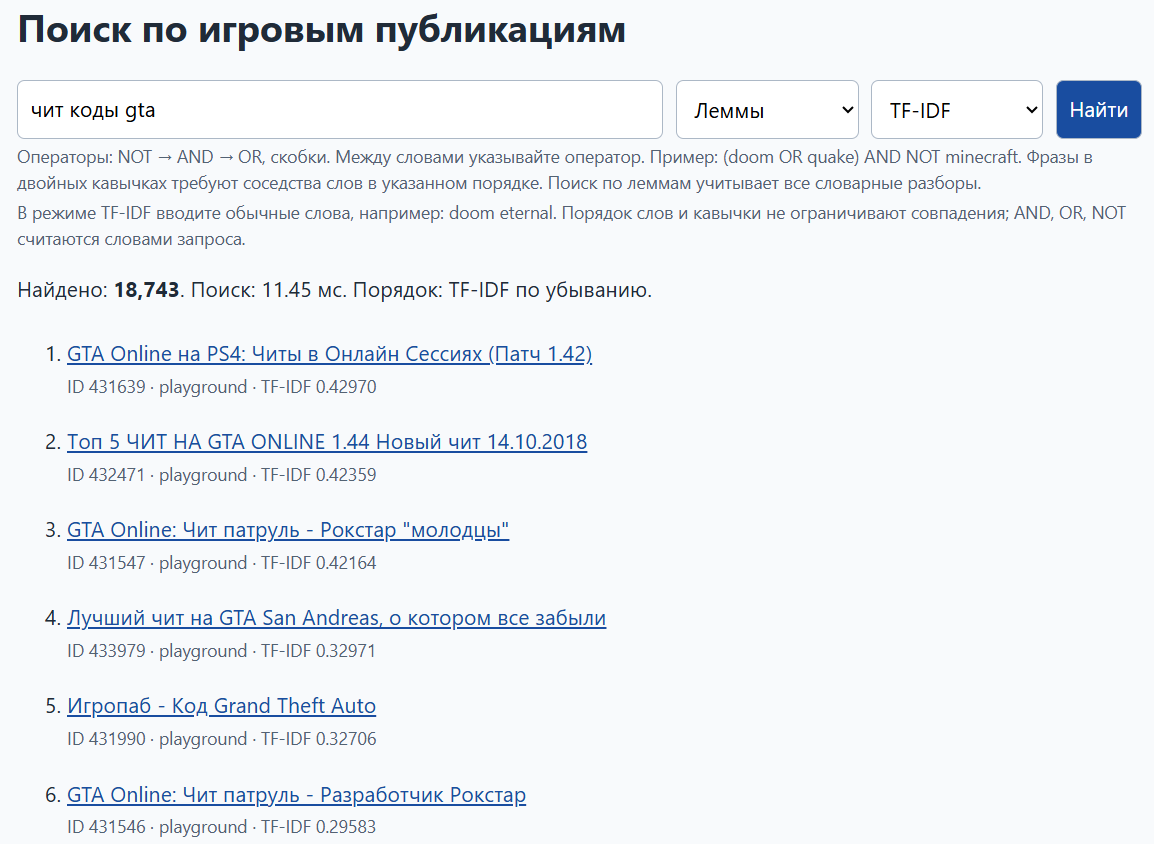
\includegraphics[width=0.96\linewidth]{img/codes_tfidf.png}
\caption{Запрос TF-IDF по леммам: 18\,743 документа с положительной оценкой}
\label{fig:codes_tfidf}
\end{figure}

Первые пятёрки TF-IDF в этих примерах состоят из публикаций
\texttt{Playground}.
Это также требует внимания: косинусная модель может высоко оценивать короткие
тексты с большой долей слов запроса. Высокая оценка не означает полноту,
актуальность или достоверность материала. Разнообразие источников,
качество содержимого и дату эта модель не учитывает.

\subsection{Воспроизводимость}
Команды сборки, построения норм, CLI и веб-формы приведены в
\path{lab13_run.md}. Скрипт \path{../run_lab13.py} сохраняет 196 измерений,
top-10, медианы, SHA-256 входов и результаты оценки по сохранённой разметке.
Исходные данные эксперимента находятся в \path{lab13/}.

Исходный код:
\href{https://github.com/kirbasss/MAI-IR/tree/lab13}{github.com/kirbasss/MAI-IR/tree/lab13}.
\begin{figure}[H]
\centering
\begingroup
\hypersetup{urlcolor=black}
\qrcode[height=25mm]{https://github.com/kirbasss/MAI-IR/tree/lab13}
\endgroup
\caption{Ссылка на ветку лабораторной работы №13}
\end{figure}

\newpage
\section{Вывод}
В этой работе я добавил ранжирование TF-IDF по схеме \texttt{lnc.ltc}.
Поисковая система принимает обычные слова и возвращает top-$k$ документов
с числовыми оценками. Независимые автотесты подтвердили расчёт косинуса,
порядок выдачи и одинаковую работу с исходным и сжатым индексами.

На рассмотренных запросах TF-IDF поднял тематические публикации в первые
строки выдачи даже при сравнении с более строгим булевым AND.
При этом поиск стал дороже: например, для \texttt{god of war} медиана
увеличилась с 15,757 до 135,160 мс. Нормы потребовали всего 7,66 МБ,
но извлечение частот из длинных координатных списков занимает время.
Его можно уменьшить, если сохранять TF непосредственно в постингах.

Полученная модель пока не учитывает порядок слов, разные веса полей
и контекст неоднозначных лемм. В выдаче заметно преимущество коротких
публикаций; небольшая оценка по заголовкам не заменяет разметку полных
документов. Дальше имеет смысл расширить набор запросов, сравнить
модели нормировки и отдельно исследовать влияние длины текста на результат.
\end{document}
